\chapter{Infraestructura}
\label{cap:infra}

En este capítulo describiremos la infraestructura utilizada, tanto software como hardware, detallando los pasos a seguir si se desea emular. En caso de que algún componente haya sido elegido entre otros de igual aplicación, expondremos las razones de la elección.


\section{Entorno}\label{sec:entorno}
Teniendo el cuenta el carácter educativo de este Trabajo, y su pretendida aplicación en estudiantes de Educación Primaria, se ha elegido el sistema operativo Windows, un entorno conocido, amigable y fácilmente accesible, para instalar y utilizar las diferentes herramientas software. \\
Tradicionalmente, cuando se hablaba de programación y especialmente de programación robótica, siempre se ha utilizado el sistema operativo Linux. Éste daba la posibilidad de instalar todos los paquetes de lenguajes de programación y entornos, mientras que Windows era especialmente cerrado en cuanto a lenguajes no nativos (fuera de \textit{bash} o de \textit{visual basic}, se hacía complicado utilizar un lenguaje de programación sin acabar recurriendo a virtualizar una máquina Linux), y los entornos software (aplicaciones) de terceros diseñados para programar habitualmente no tenían una versión instalable para Windows. \\
Sin embargo, los últimos años el Sistema Operativo se ha abierto a esta operativa, ya que la política popular demandaba poder utilizarlo, siendo el sistema operativo más utilizado por usuarios, como herramienta de desarrollo también a nivel usuario. La nueva línea de comandos de Windows, \textbf{\textit{Powershell}} (también lenguaje de scripting), añadió a la original \textit{Bash} características nativas de Linux, siendo una herramienta de programación además de administración. De hecho, en la última versión, está disponible para el propio SO de Linux (en algunas distribuciones). \\
Al principio de este Trabajo, se consideró a Linux un entorno menos amigable para usuarios sin experiencia en programación, y de la edad comentada anteriormente, por ser considerado "no de usuario": en el poco probable caso de que un estudiante conociera el sistema, lo consideraba algo muy complejo y no accesible para su nivel. Por tanto, elegir Windows eliminaba ese prejuicio y contaba con la ventaja de predisponer positivamente al alumno y de facilitarle el acceso al entorno. 

\section{Hardware}\label{sec:hardware}
En esta sección describiremos los componentes hardware utilizados. La razón de la elección de éstos responde a la misma filosofía que en la sección anterior, la facilidad de acceso a los componentes y la facilidad con que se complementa en el entorno.
\subsection{Placa Arduino}\label{subsec:placaBase}
Las placas Arduino son las más extendidas en cuanto a robótica. Arduino nació como una solución barata con el principal objetivo de utilizarlo en Educación. Además, al ser un proyecto liberado al público, su uso está extendido a toda una comunidad, que amplía y comparte sus propios desarrollos (\cite{arduinoURL}).\\
Estas placas son hardware libre (uno de las principales razones de su bajo coste), y contienen un procesador re-programable y una serie de pines hembra, donde se conectarán los periféricos de entrada/salida necesarios para controlar un robot. Hay diferentes modelos de placas Arduinos, cada una fabricada con un propósito diferente; en este caso, hemos utilizado el modelo mCore, basado en \href{https://arduino.cl/producto/arduino-uno/}{Arduino Uno}, ya que es la que lleva por defecto el robot educativo Mbot (que comentaremos en la sección \ref{subsec:mbot}). Además de los pines hembra, o puertos, contiene una serie de actuadores y sensores integrados en la placa.
\begin{figure}[H]
		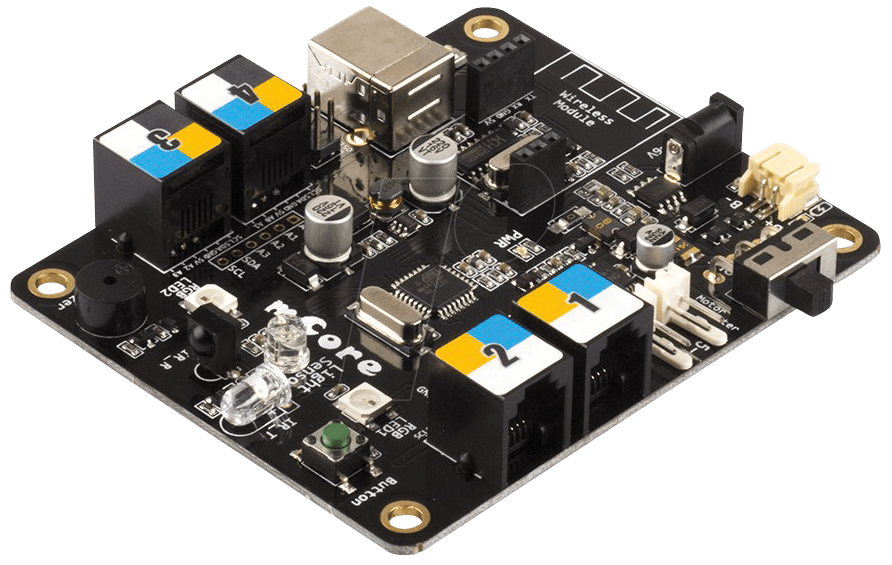
\includegraphics[width=8cm]{mcore.png}\centering
	\label{img:Mcore}
	\caption{Placa mCore}
\end{figure}
\subsection{MBot}\label{subsec:mbot}
Actualmente hay una gran variedad de robots educativos, orientados principalmente a los alumnos más jóvenes. El objetivo de la robótica educativa es ofrecer un entorno amigable y divertido, además de \textit{más realista} que la programación tradicional. Es más fácil para un niño o niña sentirse interesado por algo que tiene una reacción \textit{visible}, en algo que puede tocar y manejar, que en la programación normal que, aunque produce una reacción, es mucho más abstracta. Esto convierte la robótica en la herramienta perfecta para enseñar lenguajes, conceptos básicos de programación como funciones, uso de variables, y avanzar hasta la algoritmia se hace un proceso natural al que los propios alumnos llegan ellos mismos. \\
El principal problema al que nos enfrentamos para enseñar programación a los más jóvenes son los lenguajes de programación. Son poco intuitivos y legibles, sumado a la dificultad de mantener la atención de un alumno o alumna tan joven escribiendo en un ordenador en estos lenguajes. Era necesaria, por tanto, una forma de enseñar estos conceptos de programación comentados anteriormente sin tener que utilizar lenguajes clásicos de programación, al menos para los alumnos más jóvenes. La solución fue la programación por bloques de \textit{pseudocódigo}. El pseudocódigo es un \textit{framework}, una carcasa, que recubre el verdadero lenguaje de programación de la placa del robot, y lo hace legible y entendible. Además, siendo esto una de las grandes ventajas añadidas, la mayoría de los pseudocódigos están en casi todos los idiomas, permitiendo a los alumnos programar en su propio idioma. \\
\par Esto nos lleva al robot Mbot (\cite{makeblock}). Está basado en una placa Arduino Uno, y pensado especialmente para la enseñanza: los diferentes sensores y actuadores (los que vienen en el paquete básico, aunque hay muchos más posibles del mismo fabricante)están pensados para ofrecer prácticas entretenidas y, lo más importante, con diferentes niveles de dificultad, por lo que se puede utilizar con alumnos de diferentes edades y, durante un mismo curso escolar, crear prácticas con las que evolucionar en los conceptos. 
\begin{figure}[H]
	\includegraphics[width=8cm]{Mbot.jpg}\centering
	\label{img:mbot}\caption{Modelo Mbot utilizado}
\end{figure}
Este robot Mbot se programa utilizando un  lenguaje llamado \textit{Scratch} (\ref{subsec:scratch}),  un pseudo código muy gráfico y sencillo pero potente, que ''recubre'' la placa base. Sin embargo, al ser una placa Arduino y por lo tanto, reprogramable, siempre se puede programar en el propio lenguaje Arduino. Esto  se comentará en profundidad más adelante, en el punto \ref{cap:PyBoKids}. \\
Como se puede observar en la imagen, el robot cuenta con dos motores conectados a la placa; contiene además cuatro puertos a los que poder conectar diferentes periféricos con los que trabajar (numerados del uno al cuatro), sin contar con los motores. El modelo mostrado es el básico, sin embargo se pueden cambiar los componentes, añadiendo y/o cambiando la estructura base, y crear ''otro'' robot (por ejemplo, en las figuras siguientes \ref{img:mbot2} ). Aunque en este Trabajo de Fin de Grado solo trabajaremos con la versión básica del Mbot, esta posibilidad de añadirle componentes o cambiarlos es muy interesante para los alumnos, ya que trabajan la mecánica y pueden utilizar más tipos de periféricos.
\begin{figure}[H]
	\includegraphics[width=6cm]{Mbot-pack-piernas.jpg}
	\includegraphics[width=6cm]{Mbot-pack-piernas2.jpg}
	\centering
	\label{img:mbot2}\caption{Posibles cambios en el Mbot}
\end{figure}
\subsubsection{Sensores}\label{ssubsec:sensores}
En robótica un \textit{sensor} es un periférico de entrada que, conectado a una placa base, recoge información del medio (cantidad de ruido, temperatura, distancia frontal, etc) y la envía a la placa, dejándola disponible para toma de decisiones. La cantidad de información que se pueda recibir sólo depende de la cantidad de sensores que se pueda conectar a la vez a la placa (cuatro, en este caso, si solo se trabajara con sensores y ningún actuador). En el robot básico (de la imagen \ref{img:mbot}) los sensores son:
\begin{description}
	\item [Sensor de ultrasonidos] Está colocado en el frente, y recoge información de \textbf{distancia} hasta un objeto, en \textit{cm} (el valor máximo es 400)
	
	\item [Sensor infrarrojo \textit{Sigue Líneas}] Está ubicado de tal forma que lea, del ''suelo'', si el sensor está tapado o no, es decir: está sobre blanco o negro (de fondo, es un sensor binario). Se compone en realidad de dos sensores, izquierdo y derecho, por lo que habrá cuatro posibilidades, cada una codificada con un valor numérico (el valor que devuelve el sensor a la placa Arduino):
	\begin{itemize}
		\item Ningún sensor tapado: 0
		\item Sensor izquierdo tapado y derecho no: 1
		\item Sensor derecho tapado e izquierdo no: 2
		\item Los dos sensores tapados: 3
	\end{itemize}
	 \item [Sensor de Luz] En este caso, está integrado en la placa, por lo que no es necesario utilizar un puerto para él. Nos da un valor de cantidad de luz en el ambiente, pudiéndolo utilizar para saber si hay más o menos luminosidad de la deseada. Por supuesto, para este valor ''deseado'' será necesario obtener un valor inicial de la habitación en la que nos encontremos, para poder establecer ese valor barrera (\textit{threshold})
\end{description}
\begin{figure}[H]
	\begin{center}
		\begin{subfigure}
			[Ultrasonidos: sensor de distancia]{
			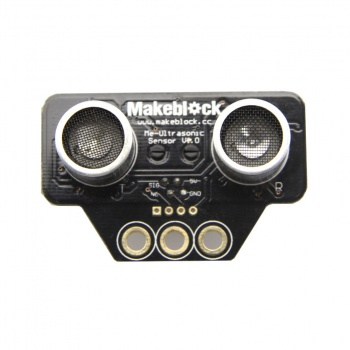
\includegraphics[width=0.45\textwidth]{ultrasonidos.jpg}
			\label{img:ultrasonidos}}
		\end{subfigure}
		\begin{subfigure}
			[Infrarrojos: sensor siguelíneas]{			
			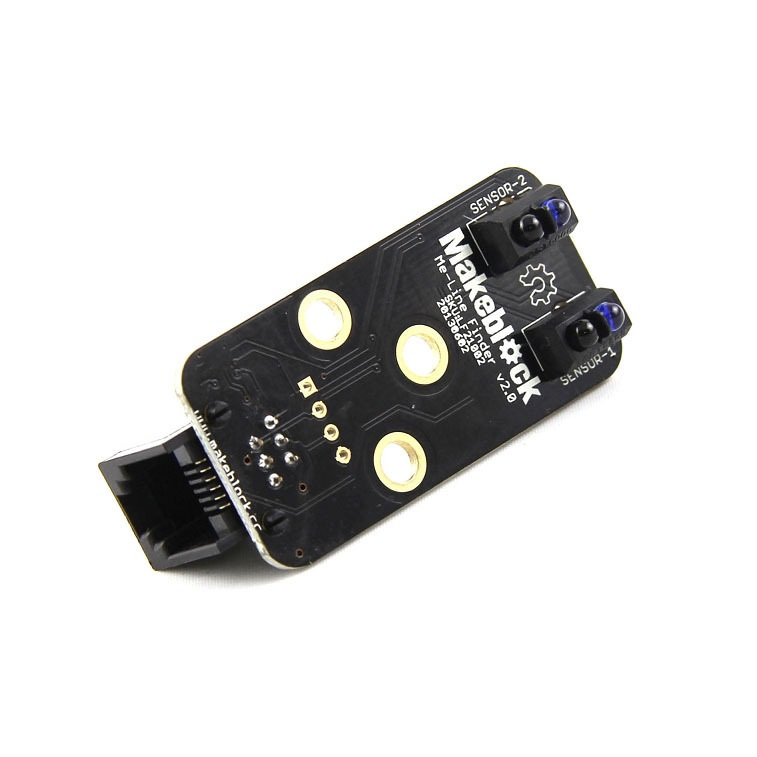
\includegraphics[width=0.45\textwidth]{siguelineas.jpg}
			\label{img:siguelineas}}
		\end{subfigure}
		\begin{subfigure}
			[sensor de luz integrado]{			
			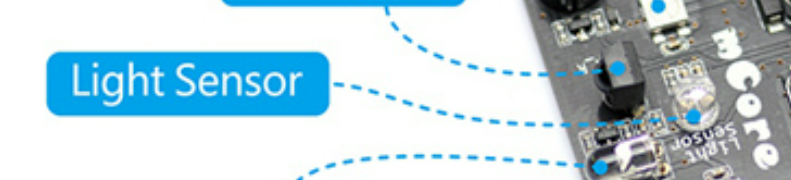
\includegraphics[width=0.45\textwidth]{sensorLuz.png}
			\label{img:sensorluz}}
		\end{subfigure}
	\label{img:sensores}
	\caption{Sensores}
	\end{center}
\end{figure}


\subsubsection{Actuadores}\label{subsec:actuadores}
	La definición de \textit{actuador} es un periférico de salida al que la placa envía datos con los que éste realiza una acción de una forma u otra. Por ejemplo, teniendo una velocidad $v_0$, este valor es enviado a los motores, que se moverán a esa velocidad y no a otra. \\
	Los actuadores, los que no están integrados en la placa directamente, se conectan a la placa a través de los mismos puertos que los sensores. Para poder usarlos, habrá que especificarle a la placa en qué puerto están conectados (igual que con los sensores). En nuestro robot básico, tenemos los siguientes actuadores:
	\begin{description}
		\item [Leds]. Están integrados en la placa, en la parte superior, y compuesto por dos led individuales que poder combinar dependiendo de qué valor codificado se envíe a la placa:
		\begin{itemize}
			\item Los dos led: 0
			\item Sólo led derecho: 1
			\item Sólo led izquierdo: 2
		\end{itemize}
		Los led son RGB (\textit{[red, green, blue]}), y el color de los dos led se codifica con un valor entre 0 y 255 para cada uno de los colores rojo, verde y azul. Así, por ejemplo, el rojo completo sería [0,255,0], el morado sería [255,0,255], el negro [0,0,0] o el blanco [255,255,255]. Estos led están codificados con valores decimales, en vez de hexadecimales como sería una codificación RGB tradicional, para facilitar la programación a los alumnos, que no conocerían el sistema hexadecimal.
		\begin{figure}[H]
			\includegraphics[width=3cm]{RGBled.png}
			\centering
			\label{img:led}
			\caption{Led RGB integrados}
		\end{figure}
		\item [Motores] En el paquete básico tenemos dos motores DC (de corriente continua) conectados a la placa en un conector específico para motores a los que conectar los dos cables, positivo y negativo. Los motores admiten como velocidad de entrada valores enteros entre [-255,255] (valores negativos para retroceder y positivos para avanzar), pudiendo dar valores diferentes a cada uno de ellos (para tener capacidad de hacer girar al robot).
		\begin{figure}[H]
			\begin{center}
				\begin{subfigure}
					[Puerto de conexión de los motores]{
						\includegraphics[width=0.45\textwidth]{puertomotor.png}
						\label{img:puertomotor}}
				\end{subfigure}
				\begin{subfigure}
					[Motor DC]{			
						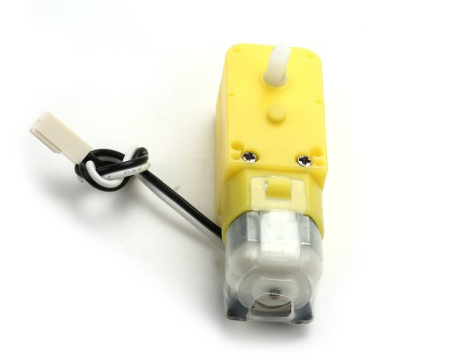
\includegraphics[width=0.33\textwidth]{motorDC2.png}
						\label{img:motor1}}
				\end{subfigure}
				\begin{subfigure}
					[Motor DC: montaje con rueda]{			
						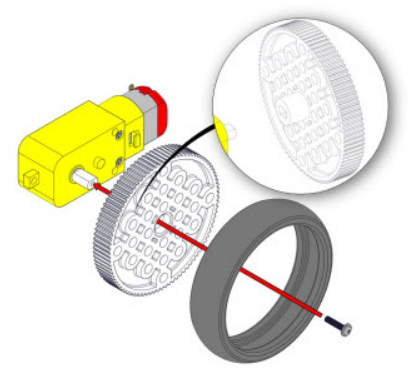
\includegraphics[width=0.33\textwidth]{motorDC.png}
						\label{img:motor2}}
				\end{subfigure}
				\label{img:motores}
				\caption{Motores}
			\end{center}
		\end{figure}
	
	\item [Zumbador] También integrado en la placa, emite notas musicales codificadas en nomenclatura americana. La equivalencia, que los alumnos necesitan conocer, está en la tabla siguiente. Para utilizar diferentes notas más agudas o más graves, se utilizan números a continuación de las letras (\textbf{C0} es más grave que \textbf{C5}). Internamente, el zumbador entiende valores enteros, correspondientes en frecuencia con cada nota (en la tabla, sólo se pone el valor para los valores \textit{1}, a modo de ejemplo):
	\begin{table}[h]
		\centering
		\begin{tabular}{ c | c | c}	
			Europea & Americana & Valor entero \\
			\hline			
			Do & C & 33\\
			RE & D & 37\\
			MI & E & 41\\
			FA & F & 44\\
			SOL & G & 49\\
			LA & A & 55\\
			SI & B & 62\\
		\end{tabular}
	\label{table:notasZumbador}
	\caption{Relación entre notas para el Zumbador del mBot}
	\end{table}

	
	\begin{figure}[H]
		\includegraphics[width=3cm]{buzzer.png}
		\centering
		\label{img:zumbador}
		\caption{Zumbador integrado}
	\end{figure}
\end{description}



\section{Software}\label{sec:software}
En esta sección describiremos el diferente software utilizado y el propósito de éste en el marco de este Trabajo Fin de Grado. 

\subsection{Scratch y mBlock}\label{subsec:scratch}
Como se ha comentado anteriormente, el robot Mbot es programable con Scratch, un lenguaje de \textbf{programación por bloques}. Un \textit{bloque de código} consiste en codificar en un ''paquete'' una sentencia completa de lenguaje (del lenguaje correspondiente, Arduino en este caso). Así, el estudiante que utilice Scratch, será capaz de utilizar una sentencia \textit{if..else} o un bucle \textit{for} de forma muy fácil y entendible, sin necesitar aprenderse todas las reglas de sintaxis del lenguaje real. A continuación, se muestran algunos ejemplos de bloques en Scratch correspondientes a los conceptos de programación más utilizados:
\begin{figure}[H]
	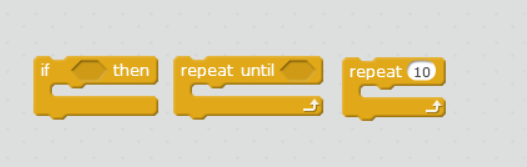
\includegraphics[]{scratch.png}
	\centering
	\label{img:scratch}
	\caption{Algunos ejemplos de bloques en Scratch}
\end{figure}
Como puede observarse, las sentencias que se quieran repetir, o las variables de condición, tienen un lugar muy intuitivo donde colocarse. Además, pueden crearse variables, en las que guardar los valores de los sensores y poder utilizar como entrada de actuadores, o como valores de referencia. \\
Ciertamente, y aunque el lenguaje Scratch puede utilizarse como lenguaje de programación ''tradicional'', utilizando un escenario virtual con un personaje para observar el resultado del programa (sin robot físico), es mucho más completo al añadirle el módulo del robot deseado. Este módulo contiene bloques para recoger valores de los sensores o enviar valores a los actuadores, ya sean \textit{''on board''} (integrados en la placa), o teniendo que especificar el puerto al que están conectados:
\begin{figure}[H]
	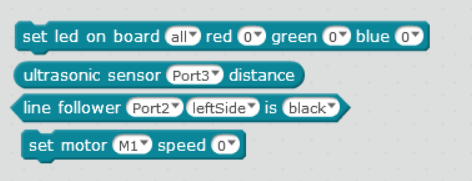
\includegraphics[]{scratch2.png}
	\centering
	\label{img:scratch2}
	\caption{Ejemplos de bloques de Mbot en Scratch}
\end{figure}

Para utilizar Scratch y programar el robot, es necesario instalar un programa, que es el que contiene el compilador y el que permite conectar el robot al PC para enviarle el programa, llamado \textit{mBlock}. El ejecutable se descarga de la página oficial del fabricante, \href{https://www.makeblock.es/blog/descargas/}{Makeblock}, disponible para PC (también existe una versión simplificada para dispositivos móviles).\\
Una vez instalado el software, el proceso para poder empezar a usar el mBot es muy simple:
\begin{enumerate}\label{list:conexionMblock}
	\item Conectar el robot al pc con el cable USB, y conectarlo con el programa (el robot debe estar encendido).
	\begin{figure}[H]
		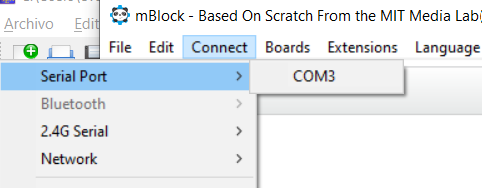
\includegraphics[]{mblock.png}
		\centering
		\label{img:mblock}
		\caption{Conectar el mBot}
	\end{figure}

	\item  Asegurarse de que la placa corresponde con el robot que tenemos
	\begin{figure}[H]
		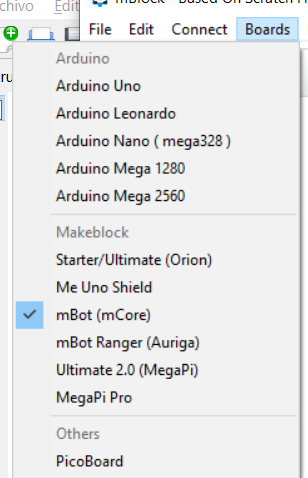
\includegraphics[]{mblock2.png}
		\centering
		\label{img:mblock2}
		\caption{Placa mBot}
	\end{figure}

	\item Actualizar el programa Arduino subido a la placa base, para que funcione con Scratch (en caso de haber utilizado el robot con otro programa)
	\begin{figure}[H]
		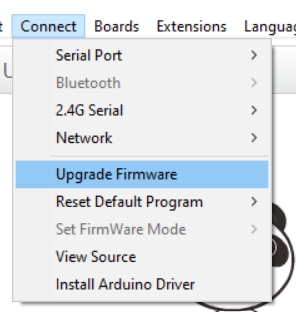
\includegraphics[]{mblock3.png}
		\centering
		\label{img:mblock3}
		\caption{Actualizar firmware de la placa}
	\end{figure}

	\item Una vez programado algo de código, para subirlo al robot: click derecho sobre el código, 'upload to arduino', para compilar el programa, y otra vez a 'upload to arduino' cuando el compilador aparezca en la parte derecha de la pantalla, para subirlo a la placa
	\begin{figure}[H]}
		\centering
		\begin{subfigure}
			[Compilar programa]{
				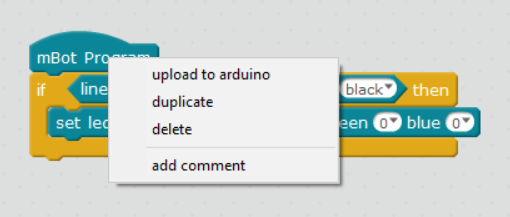
\includegraphics[width=0.45\textwidth]{mblock4.png}
				\label{img:uploadArduino1}}
		\end{subfigure}
		\begin{subfigure}
			[Subir programa a la placa]{
				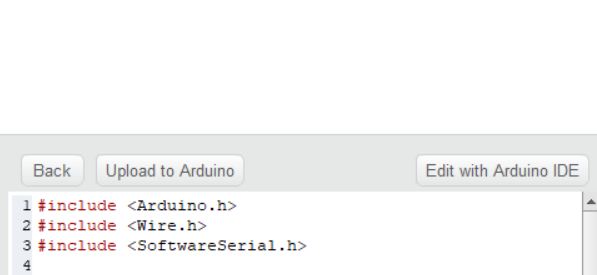
\includegraphics[width=0.5\textwidth]{mblock5.png}
				\label{img:uploadArduino2}}
		\end{subfigure}
	\caption{Subir programa a la placa del mBot}
	\end{figure}

	\item Una vez subido el programa, el robot comenzará a funcionar tal y como lo hayamos programado.
\end{enumerate}
 

\par Este lenguaje, junto a la interfaz gráfica, es una perfecta primera aproximación a la programación y a la robótica, dando más importancia al aprendizaje conceptual que a la sintaxis y al lenguaje. \\
Obviamente, los alumnos necesitarán que se les guíe, principalmente al comienzo del curso, en comprender las necesidades de incluir los diferentes bloques y las ventajas que produce en el código. El objetivo no será explicarles para que usar, por ejemplo, un bloque condicional,  sino proponerles un ejercicio en el que, para llegar a la solución, necesitarán de forma intuitiva programar un condicional, y lleguen naturalmente a la necesidad de ello.
\subsection{Arduino}\label{subsec:arduino}
Como se explicó cuando hablamos de la placa base en la sección \ref{subsec:placaBase}, ésta se programa en \textbf{Arduino}. Este lenguaje de programación está basado en C++, y pensado para interactuar con objetos electrónicos. \\
Teniendo en cuenta el objetivo de este Trabajo Fin de Grado, ofrecer una posibilidad de programar el robot Mbot en Python, es necesario utilizar el lenguaje nativo de la placa base, con el fin de que el robot \textit{entienda} las órdenes programadas en Python. Por lo tanto, para crear este ''framework'', es necesario instalar el entorno Arduino. A continuación se explican las instrucciones para instalar el entorno en Windows, y para configurarlo para el robot.
\begin{enumerate}\label{list:InstalacionArduino}
	\item Descargar e instalar, Arduino IDE, el cual instala el entorno completo de Arduino. Para las versiones 8 y 10 de Windows, está disponible directamente en el Microsoft Store. Para otras versiones de Windows, está disponible en la  \href{https://www.arduino.cc/en/software}{página web oficial}.
	\begin{figure}[h]
		\includegraphics[width=10cm]{store.png}
		\centering
		\label{img:MStore}
		\caption{Arduino IDE en el Microsoft Store}
	\end{figure}
	\item Descargar las librerías de \href{https://codeload.github.com/Makeblock-official/Makeblock-Libraries/zip/master}{Makeblock} o del \href{https://github.com/JdeRobot/PyBoKids/tree/main/PyBoKids%202.0}{repositorio PyBoKids} para añadirlas a Arduino y poder utilizarlas en nuestro entorno.
	\item Incluir el archivo comprimido descargado desde el Arduino IDE:\\ \textit{Programa - Incluir librería - Añadir biblioteca .ZIP - Seleccionar el fichero - Abrir}
	\item Seleccionar la placa básica que se va a conectar al IDE:\\
	\textit{Herramientas - Placa - Seleccionar Arduino Uno}
	\item Especificar el modelo exacto de placa al principio del programa de Arduino; en este caso la placa que estábamos utilizando es la mCore. Así se cargan todos los métodos correspondientes al modelo de placa; debe incluirse en cada programa de Arduino que se escriba.
	\begin{verbatim}	
		#include "MeMCore.h"	
	\end{verbatim}
	\item Igual que con Scratch, primero se debe conectar el robot al software (con el robot enchufado al PC y encendido):\\
	\textit{Herramientas - Puerto - Seleccionar el puerto en el que está el robot} \\
	Los puertos USB en Windows son \textit{COM1, COM2, COM3}, etc.
	\item  Una vez tengamos un programa en Arduino listo para subir a la placa y probar con el robot:\\
	\textit{Programa - Subir } o el botón rápido de ''subir''. \\
	Este proceso primero compilar el programa y, si está correcto, lo sube a la placa. Sin embargo, se puede compilar primero como comprobación \textit{(Programa - Verificar)}.
\end{enumerate}
\subsection{Python}\label{subsec:python}
Por último, utilizaremos \textbf{python} para programar la lógica de los ejercicios. El objetivo es que se programe en python sólo los ejercicios, habiendo paquetizado todo lo relativo al robot en Arduino, y sólo utilizando la conexión con éste para obtener datos de los sensores y enviar datos a los actuadores. La descripción de este proceso y de la lógica de ambos lados (PC y robot) se describirá en profundida en el capítulo \ref{cap:PyBoKids}.
\par La razón de utilizar Python como lenguaje de programación es la misma que la del resto de componentes: la facilidad para los alumnos de acceder a ello. Es uno de los lenguajes con sintaxis más simple (por comparación, Arduino / C++ es muy cerrado y complejo), además de ser las palabras reservadas significantemente entendibles (aunque es cierto que en inglés: \textit{while}, \textit{print}, \textit{read}, etc), así como la declaración de variables es más flexible. Además, y aparte de la cuestión educacional, el módulo \textit{serial} para conexión con periféricos, está con la instalación base, y es mucho más sencillo que en otros lenguajes, haciéndolo perfecto para la electrónica. 
\par La instalación de python en Windows también es muy sencilla:
\begin{enumerate}\label{list:instalacionPython}
	\item Descargar el paquete de la \href{https://www.python.org/downloads/}{web oficia} y ejecutar el instalable descargado.
	También es posible, para Windows 10, obtenerlo desde el Microsoft Store, tal y como se hizo para Arduino.
	\item Una vez descargado, comprobar que se puede ejecutar abriendo una consola -Powershell- y escribiendo \textit{python},	se ejecutará la consola de python, y podremos probar que tenemos python instalado en nuestro entorno (\textit{exit()} para salir). También es útil comprobar que hemos instalado la versión correcta (3.10): \textit{python --version} en una consola de Powershell (no teniendo abierta la consola de python)
	\begin{figure}[h]
		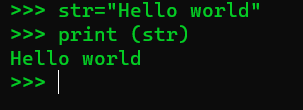
\includegraphics[]{python.png}
		\centering
		\label{img:python}
		\caption{Comprobar python}
	\end{figure}
	\item Para ejecutar un programa escrito en python desde la consola de Windows: 
	\begin{verbatim}
		py HelloWorld.py
	\end{verbatim}
	\item Es probable que la versión de Python, tanto descargada del repositorio oficial como de Microsoft Store no tenga el módulo Serial (necesario para las comunicaciones con el robot) instalado de serie. Tan solo es necesario ejecutar en Powershell la siguiente línea de código:
	\begin{verbatim}
		pip install pyserial
	\end{verbatim}
	\begin{figure}[h]
		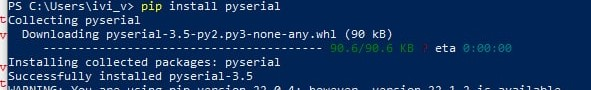
\includegraphics[]{pyserial.jpg}
		\centering
		\label{img:pyserial}
		\caption{Instalar módulo necesario en Python}
	\end{figure}
\end{enumerate}
\newpage
Para escribir código en python, se puede utilizar cualquier editor de texto. El mismo instalador de python instala uno propio, \textit{IDLE shell}, suficientemente simple y preparado particularmente para su sintaxis.
